\section{Event Representation}\label{sec:geo:model}

We introduce a novel high-level event representation, called {\em
spatio-temporal context-aware event representation}, with the purpose of gaining
insight about real-world news from social media as well as from the relations
between locations and impact that these events induce. 
%
Specifically, we define our event representation and how it can be used to study
relations among locations.

\subsection{Event Representation Definition}\label{sec:model_definition}

We extend our previous definition of an event to a complex information unit that
encompasses all of the available social media content associated with a certain
news topic, as well as its aggregated spatial and geographical information.
%
%Events are represented
%as: i) the set of {\em keywords} that describe a particular news topic,
%and ii) the set of all of the {\em social media messages} that discuss the
%event, posted during the timeframe of its occurrence.
%
%We modify the aforementioned model by adding spatial and temporal context of
%the event's high-level abstraction.
%
In particular, we incorporate information about the locations involved in the
event occurrence, and the locations of the users that post messages about the
event. 
%
This representation is solely based on the social media activity surrounding the
event in the online social network, without including any external information
sources.
%
Specifically, we define two types of spatial contexts, which we call:
\begin{enumerate}
\item {\bf protagonist locations}, which are the locations involved in the
event, and
\item {\bf interested locations}, which are the locations from where users
comment on the event.
\end{enumerate}

For example, consider the news about Chile and Peru's maritime dispute at The
Hague in The Netherlands~\cite{bbc_peruchile}. 
%
If we define locations at country level, then this is an event for which Twitter
users mention mostly three countries when discussing the event: Chile, Peru and
The Netherlands (other mentions are negligible). 
%
Hence, according to our definition this event is considered to have three
protagonist locations. 
%
However, users that comment on this event are located mostly in: Chile, Peru,
Argentina and Bolivia. 
%
Therefore, the event is considered to have four interested locations.

More formally, we define an event $E$ as a tuple of the form:
%
\begin{equation} \label{eq:event}
E = (K, D, T, \mathbf{P}, \mathbf{I})
\end{equation}
%
%\medskip
\noindent where $K$ is  a set of keywords, which succinctly describe the news
topic, $D$ is the date of the event detection, $T$ is a set of tweets about the
event, published by users of online social networks.
% Tweets are also defined as tuples of the form
%$t = (u, l, m, d)$ for any tweet $t \in T$, where $u$ denotes the user who posted
%$t$, $l$ denotes the location of the user $u$, $m$ denotes the message text contained in $t$, and $d$
%denotes the date when $t$ was posted.
In addition, consider $L=\{l_1, l_2,\ldots, l_{|L|}\}$ to be the set of existing
locations. 
%
We augment the information about the event by explicitly including its spatial
context with the vectors $\mathbf{P}$ and $\mathbf{I}$, which correspond to the
{\em protagonist} and {\em interested} location values, respectively, for the
event $E$. 
%
In particular, the $j$-th dimension of vector $\mathbf{P}$ contains the number of
times that the location $l_j$ is mentioned by the tweets in $T$. 
%
On the other hand, the $j$-th dimension of vector $\mathbf{I}$ contains the
number of tweets in $T$ that were posted by users in the location $l_j$.


Using the information introduced by vectors $\mathbf{P}$ and $\mathbf{I}$ we can
derive the scope of an event $E$ from two perspectives, {\em provenance} and
{\em impact}, defined as follows:
%\bp{See if these are the best names.. not sure yet}

\begin{itemize}
\item{\bf Provenance:} 
%
Indicates whether an event is local, regional or global in terms of the
locations it involves.
%
We consider an event to be of {\em local provenance} if it involves only one
protagonist location. 
%
We consider an event to be of {\em regional provenance} if it involves two or
more protagonist locations that are all from a same region (e.g., for countries,
this means neighboring countries or countries from the same continent\footnote{According to
the division that considers 7 continents: Asia, Africa, Europe, North America,
South America, Antarctica and Australia.}). 
%
We consider an event to be of {\em global provenance} if it involves two or more
protagonist locations in which at least one is not from the same region. 
%
Vector $\mathbf{P}$ contains this information for a given event $E$.


\item{\bf Impact:} 
%
Indicates if an event is local, regional or global in terms of how many
locations show interest in it. 
%
We consider an event to be of {\em local impact} if it generates conversation
from users in only one location (i.e., one interested location). 
%
We consider an event to be of {\em regional impact} if it generates conversation
from users in more than one interested location, all from the same region.  
%
We consider an event to be of {\em global impact} if it generates conversation
from users in more than one interested location in which at least one of those
locations is not from the same region. 
%
Vector $\mathbf{I}$ contains this information for a given event $E$.
\end{itemize}

For example, the message {\em ``Australia confirms signals detected by China
`consistent' w/ \#MH370 black box''}, discussed an event in which Australia and
China are involved. 
%
Therefore, Australia and China can be considered as protagonist locations in
this event. 
%
On the other hand, this particular news event was discussed extensively by users
located in several countries, including: USA, Canada, Colombia, U.K., India,
Nigeria, South Africa, Indonesia, Australia, France, Germany, China and Italy.
%
Therefore, this is an event that had {\em global provenance} (i.e., more than
one protagonist location from different regions) and {\em global impact} (i.e.,
more than one interested country from different regions).

%%

It should be noted that there can be different levels of ``global impact'',
depending on how many different locations show interest in the event (e.g., a
high-impact global world events will spark conversation in many countries). 
%
In addition, a location can be of any type of geopolitical division granularity,
such as a city, a region, a country, a continent, etc. 
%
However, for our work we focus on locations at {\em country level}. 
%
Therefore, at times we use the concepts of ``locations'' and ``countries''
interchangeably.
%
In particular, in the following section, we define a representation for
relations among locations, which we leverage in Section~\ref{sec:geo:mining} for
extracting international relations.




\subsection{Representing Relations Among Locations}\label{sec:relations}

The spatio-temporal context-aware event representation allows us to extract
different types of relationships among locations for a given event collection.
%
In particular, we define a {\em protagonist-interest} vector $\mathbf{pi}$ for a
location $l_j$, which represents the interest that other locations have in
events that have $l_j$ as a protagonist.  
%
We define $\mathbf{pi}$ for $l_j$ as:

\begin{equation} \label{eq:pi}
%\mathbf{pi}(l_j) = \langle w(l_j,l_1),w(l_j,l_2),\ldots,w(l_j,l_{|L|}) \rangle
\mathbf{pi}(l_j) = \Big[ w(l_j,l_1),w(l_j,l_2),\ldots,w(l_j,l_{|L|}) \Big]
\end{equation}
%
\noindent where,
%
\begin{equation} \label{eq:pi-w}
w(l_j,l_k)=
f(\mathit{\#~of~events~that~have}~l_j~\mathit{as~protagonist}~\mathit{in~which}~l_k~\mathit{shows~interest}),~\forall~l_j,l_k \in L
\end{equation}
%
Likewise, we also define the {\em co-protagonist} vector $\mathbf{cp}$ for the
location $l_j$ as follows:
%
\begin{equation} \label{eq:cp}
%\mathbf{cp}(l_j) = \langle w'(l_j,l_1),w'(l_j,l_2),\ldots,w'(l_j,l_{|L|}) \rangle
\mathbf{cp}(l_j) = \Big[ w'(l_j,l_1),w'(l_j,l_2),\ldots,w'(l_j,l_{|L|}) \Big]
\end{equation}
%
\noindent where,

\begin{equation} \label{eq:cp-w}
w'(l_j,l_k)=
f(\mathit{\#~of~events}~l_j~\mathit{as~protagonist}~\mathit{in~which}~l_k~\mathit{is~also~a~protagonist}),~\forall~l_j,l_k \in L
\end{equation}

The relationships between locations, given by $\mathbf{pi}$ and $\mathbf{cp}$,
allows us to identify similarity relationships among locations, such as:

\begin{itemize}
\item{\bf Locations that produce similar interest:} 
%
from $\mathbf{pi}$ we can extract sets of locations (countries) that are
similar, based on the level of interest that they produce in other locations
(countries). 
%
For example, they can be obtained using $k$ nearest neighbors or by clustering
locations' $\mathbf{pi}$ vectors.

\item{\bf Locations that are protagonists of the same events:} 
%
from $\mathbf{cp}$ we can identify which locations (countries) are similar,
based on their interactions (i.e., they are protagonists of the same event) with
other locations (countries). 
%
For example, they can be obtained using $k$ nearest neighbors or by clustering
locations' $\mathbf{cp}$ vectors.
\end{itemize}

The weights, $w(l_j,l_k)$ and $w'(l_j,l_k)$, are expressed as a function
$f(x_{j,k})$, where $x_{j,k}$ corresponds to {\em \# of events in which $l_j$
and $l_k$ interact}. 
%
In particular, for Galean, users have expressed the preference of visualizing
the {\em absolute} number of events in which two countries interact (i.e.,
$f(x_{j,k})=x_{j,k}$).  
%
Nevertheless, there are other cases in which the analyst could prefer the
weights to reflect the fraction of events in which two countries interact in
relation to the total of events for one of the two locations (e.g., where the
number of events is normalized by the amount of events in which $l_j$ or $l_k$
participates).
%
This can be useful in cases where the number of events in which different
locations participate are very concentrated on specific locations. 
%
We explore cases such as these in Section~\ref{sec:geo:mining}, where we analyze
the dataset which is biased towards certain countries.

%%

We note that weights can also be expressed as functions of the {\em \# of
tweets} or the {\em \# of users}, and in addition, the proposed representation
allows us to also specify {\em interest-interest} and {\em interest-protagonist}
vectors, in a similar fashion to $\mathbf{pi}$ and $\mathbf{cp}$. 
%
However, we do not focus on these variations in this dissertation.

\begin{figure}[h]
  \centering
  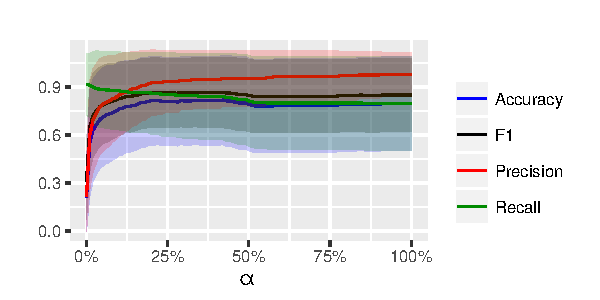
\includegraphics[width=\textwidth]{figures/geopolitical/k_accuracy_recall.pdf}
  \caption[Mean and standard deviation of multi-label scores]{Mean and standard
  deviation of multi-label scores of accuracy, precision, recall and F1 measure
  by $\alpha$ ratio for 100 randomly selected events from our dataset.}
  \label{fig:eval}
\end{figure}

\medskip
\paragraph{Precision and recall of event locations.}
%
Empirically, we observed that the precision and recall of the locations
considered to be protagonist of an event depends mostly on a ratio, which we
call $\alpha$.
%
For an event $E$ that contained more than one location, we defined $\alpha$ as
the minimum percentage of tweets that must refer to a location $l_i$ in relation
to the most mentioned location $l_{\mathrm{max}}$, in order for $l_i$ to be
included in $\mathbf{P}$ or $\mathbf{I}$ vectors.
%
Figure~\ref{fig:eval} shows an empirical analysis of the effect of $\alpha$ on
the precision, recall and $F_1$ metrics of protagonist locations on a sample of
100 events.  
%
Precision and recall were estimated based on a manual assessment of the
protagonist locations of those events. 
%
Based on this variation $\alpha$ can be set as the value that provides the best
trade-off between $F_1$ and recall ($\alpha = 19\%$ in our experiment).

In addition, if $E$ has only one location $l$, we require that this location is
mentioned a minimum percentage of tweets, which we define as $\beta$. This ratio
is also defined within the same experimental scenario, determined from the
smallest percentage of mentions that $l$ can have in relation to the total
number of tweets in $E$, for a given $\alpha$.



\subsection{System Architecture}\label{sec:framework}

We present a general overview of the architecture for generating our event
representations in order to use them in our application.  
%
The architecture, shown in Figure~\ref{fig:sys_architecture}, consists of the
following three parts: {\em ``input''}, {\em ``event representation
generator''}, and {\em ``visualization''}.  
%
The first component, (1) ``input'', is not part of the particular contribution
of this chapter\footnote{The {\it News event extractor} module is part of our
data collection methodology, as described in Chapter~\ref{chapter:data}}, and is
currently fulfilled by using existing methods, which can be replaced
transparently as long as the requirements detailed next are met. 
%
On the other hand, the other two components, (2) ``event representation
generator'' and (3) ``visualization'', are the core of our contribution and
therefore essential to our system.


\begin{figure*}[t]
    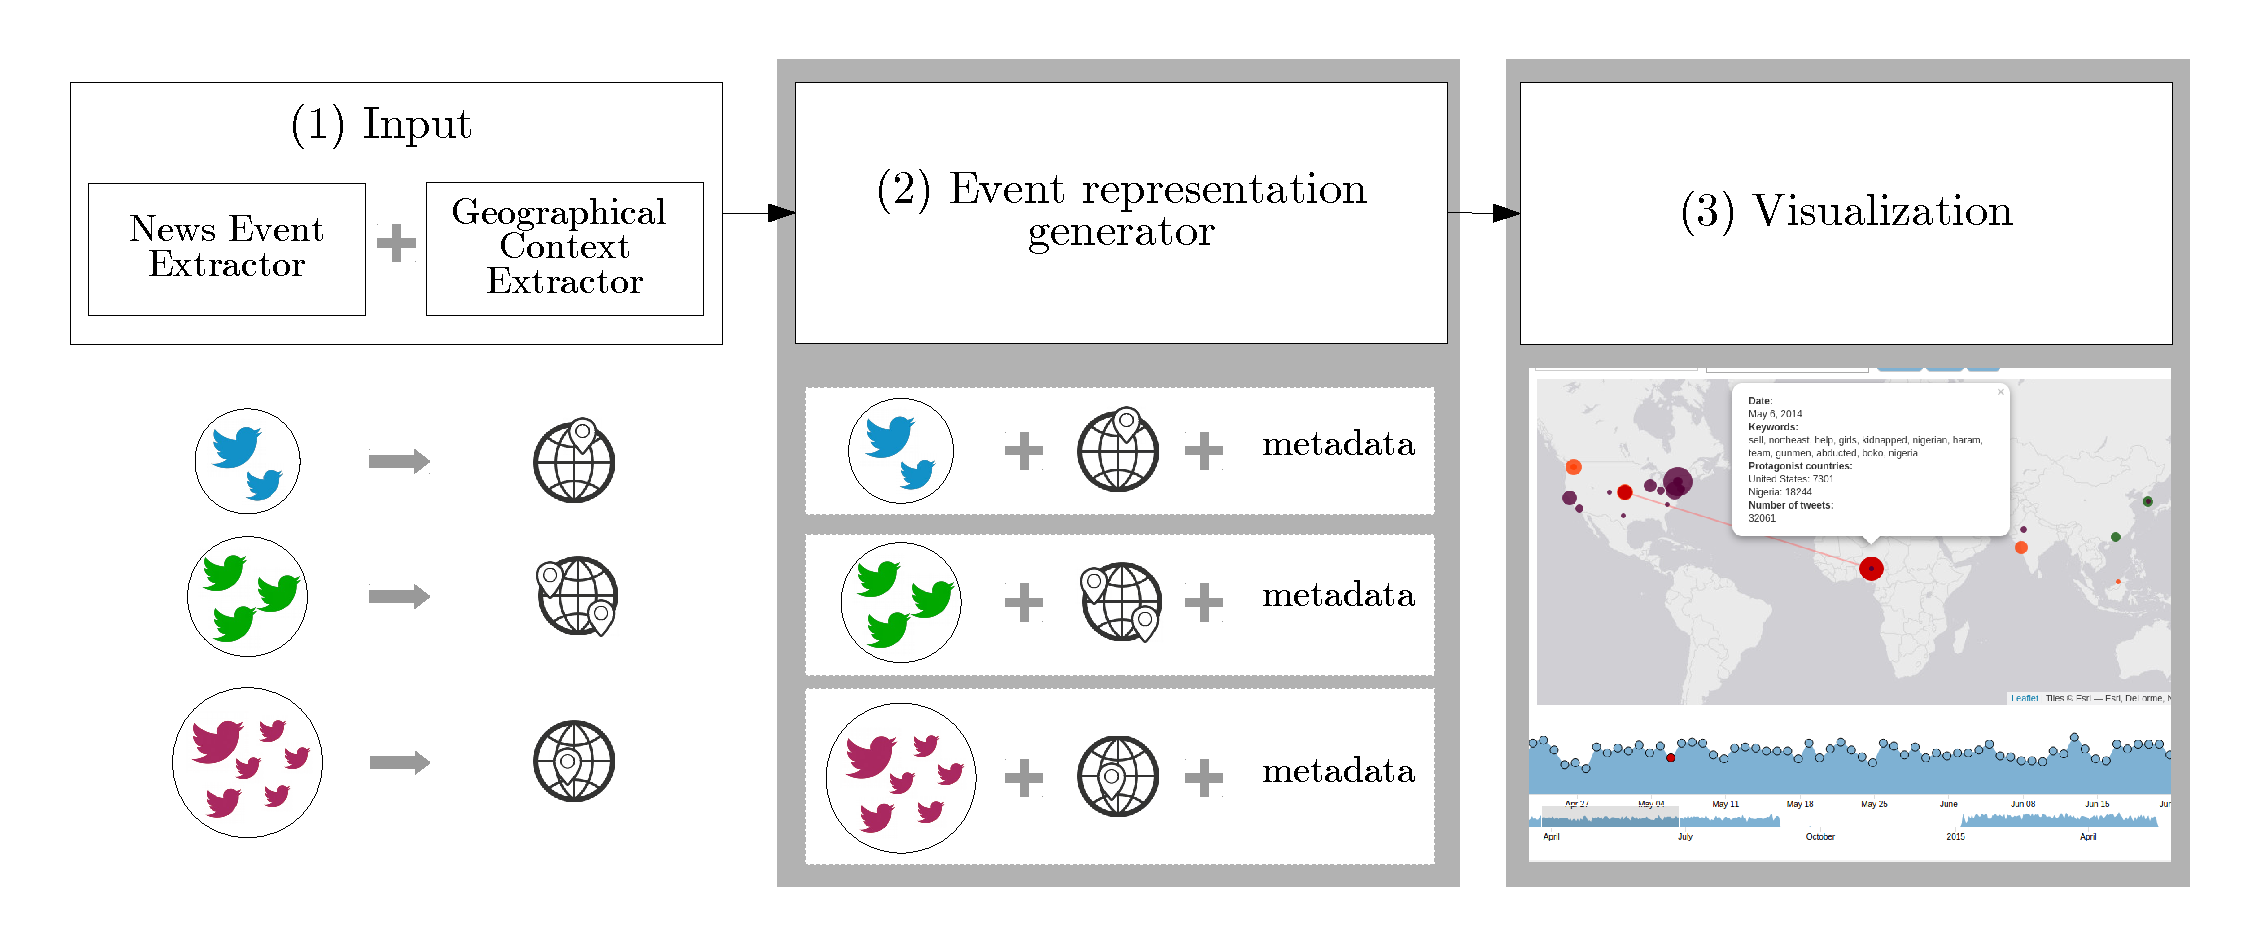
\includegraphics[width=\textwidth]{figures/geopolitical/architecture.pdf}
    \caption[Data architecture for Spatio-Temporal Model.]
    {Framework consisting of three parts: 1) input, which collects data related
    to news event activity from social media and extracts its geographical
    information; 2) the event representation generator, which generates our
    representation of the input events and 3) the visualization, which consumes
    these events. Our contribution is related to the two latter modules, the
    first module can be replaced according to the task and/or state-of-the-art.}
    \label{fig:sys_architecture}
\end{figure*}

Given an input from the Twitter data stream we specify the following components
of our framework:

%%

\begin{enumerate}

\item{\bf Input:} 
%
This module requires two sub-parts, the {\em ``news event extractor''} and the
{\em ``geographical context extractor''}.
%
    \begin{enumerate}
    %
    \item{\em News event extractor:} 
    %
    This sub-module must output groups of tweets, where each group of tweets $T$
    should represent a cohesive news topic $E$.  
    %
    In particular, most of the tweets in the set $T$ of an event $E$ must be on
    the topic of a particular news events. 
    %
    However, as we use a high-level representation of events, some noise is
    tolerated (i.e., tweets that do not correspond to the event).

    \item{\em Geographical context extractor:} 
    %
    This sub-module associates spatial context to each tweet in $T$ of each event
    $E$ produced by the ``news event extractor'' module. 
    %
    Therefore, it must provide the geographical locations of the places
    mentioned in the text of the message and the geographical location of the
    author of the message (i.e., protagonist and interested locations,
    respectively). 
    %
    This module must locate the majority of the tweets in $E$ correctly (i.e.,
    with good precision) based on GPS coordinates and/or textual content, so
    that locations mentioned in tweets can be geo-tagged, and users can be
    geo-tagged as well (users can set their location using GPS coordinates or by
    using natural text).

    \end{enumerate}
%
\item{\bf Event representation generator}: 
%
This component creates the event representations $E$ for each of the groups of
tweets provided by the ``input'' module. 
%
In particular this module is responsible for creating a tuple $E$ for each
event, as specified by our definition in Section~\ref{sec:model_definition}.
%
This means that it has to produce the date $D$ of the first tweet, a set of
keywords $K$ that describe the event, the set $T$ of tweets and the $\mathbf{P}$
and $\mathbf{I}$ location vectors of the event.

%%

\item{\bf Visualization}: 
%
This module consumes the event representations
produced by the ``event representation generator'' module and produces the event
visualization interface.

\end{enumerate}



\noindent{\bf News event extraction setup.} 
%
The news event extraction module corresponds to that proposed in
Chapter~\ref{chapter:data}, which consists of an ongoing process that
periodically retrieves tweets about real-world news. 
%
The process produces coherent sets of tweets about news topics, although with a
certain degree of noise that is well tolerated by our system. 
%
In particular, this is a two-stage iterative process that consists of the
following steps:
%
(1) {\em news topic identification} (i.e., detection), and 
%
(2) {\em event tweet extraction}. 


\smallskip
\noindent{\bf Geographical context extraction setup.}
%
We create a methodology for extracting the protagonist and interested locations,
as well as their frequency for an event $E$ with a set of tweets $T$.  
%
The {\em toponym} (i.e., location name) extraction and resolution phases are
carried out using the off-the-shelf geo-parser, CLAVIN~\cite{clavin}. 
%
However, since tweets are short and do not provide much context for toponym
disambiguation, our methodology boosts the performance of the geo-parser by
adding context from other tweets in $E$.

As detailed in Section~\ref{sec:geo:model}, this methodology relies on a ratio
named $\alpha$ which we empirically set to $19\%$ as that which provides the
best trade-off between F1 and recall, according to Figure~\ref{fig:eval}. 
%
In other words, a location must have at least $19\%$ of the mentions of the most
frequent location of an event, to be considered as part of that event as well.
%
Otherwise, we consider that this location was not actually involved in the
event.

